\chapter{Metodología y preparación de datos}
\label{cap:pre_datos}
\begin{resumen}
	En este capítulo describimos la metodología seguida para procesar y transformar las señales de ECG de la base de datos PTB-XL, detallamos la distribución de las clases, el preprocesamiento aplicado, las transformaciones realizadas y las métricas empleadas para evaluar los modelos.
\end{resumen}

\section{Análisis de los datos y distribución por clases}
La base de datos PTB-XL es un conjunto de registros formado por 21799 ECGs de 12 derivaciones, considerado uno de los mayores \emph{datasets} públicos de ECGs disponibles en la actualidad \citep{ptbxlart}. Contiene muestras de ECGs de 10 segundos de duración anotadas con múltiples etiquetas diagnósticas. Para este trabajo, emplearemos la clasificación según las superclases definidas en la propia base de datos, que coinciden con las que presentamos en la Sección \ref{subsec:anomalias}.

La Tabla \ref{tab:dist} muestra la distribución de los datos de PTB-XL considerando estas cinco superclases. Se observa que la clase ``NORM'' es la más numerosa, mientras que la clase ``HYP'' tiene una cantidad considerablemente menor de datos. Este desbalanceo de clases puede causar varios problemas en el modelo, como por ejemplo:

\begin{table}[t]
	\centering
	\begin{tabular}{|lllr|}
		\hline
		Número de registros & Superclase & Descripción & Porcentaje \\
		\hline
		9514 & NORM & ECG Normal & 43.64\% \\
		5469 & MI & Infarto de Miocardio & 25.08\% \\
		5235 & STTC & Cambio ST/T & 24.01\% \\
		4898 & CD & Transtorno de la conducción & 22.46\% \\
		2649 & HYP & Hipertrofia & 12.15\% \\
		\hline
		
	\end{tabular}
	\caption{Distribución de las superclases en PTB-XL}
	\label{tab:dist}
	\begin{tablenotes}
		\small
		\item La información de esta tabla ha sido extraída directamente del \href{https://physionet.org/content/ptb-xl/1.0.3/}{repositorio de PTB-XL}.
	\end{tablenotes}
\end{table}

\begin{enumerate}
	\item \textbf{Sobreajuste hacia la clase mayoritaria:} Al haber bastantes más datos de entrenamiento de una clase (NORM) y menos de otra (HYP), el modelo puede aprender mejor los patrones que identifican las clases mayoritarias, haciendo que sepa distinguir peor las minoritarias, lo que en este caso podría reducir notablemente su capacidad de predicción de anomalías raras \citep{IData}.
	
	\item \textbf{Métricas no representativas:} Las métricas más comunes, como la exactitud, pueden ser poco informativas cuando hay un desbalance en los datos de prueba, ya que un modelo que predice siempre la clase mayoritaria puede tener una exactitud alta. Esto puede dificultar la evaluación real del rendimiento del modelo \citep{ClassOfIData}.
	
	\item \textbf{Dificultad en el entrenamiento:} Las redes neuronales profundas requieren de grandes cantidades de datos de entrenamiento para poder entender patrones complejos. Si una de las clases tiene muy pocos ejemplos, es muy probable que el modelo no sea capaz de predecirla correctamente \citep{Leevy}.
\end{enumerate}

Para abordar estos problemas existen varias estrategias, como hacer \emph{oversampling} o \emph{undersampling}. El \emph{oversampling} consiste en generar datos sintéticos a partir de los que ya tenemos para balancear las clases \citep{he2008adasyn}, pero esto no es una buena técnica cuándo los datos son complejos (como es el caso de un electrocardiograma), ya que no hay una técnica clara para crear datos sintéticos coherentes. Por otro lado, el \emph{undersampling} hace que todas las clases se queden con el mismo número de candidatos que la clase minoritaria, lo que no es una técnica adecuada cuándo los datos de entrenamiento son reducidos desde un principio \citep{koziarski2019radial}.

\section{Preprocesamiento de datos}
\label{sec:procesamiento}
En cualquier desarrollo de IA, antes de poder utilizar los datos hay que hacer cierto procesamiento para asegurarnos que son adecuados. Lo primero que habría que hacer es quitar los datos repetidos, incompletos o corruptos, pero afortunadamente la base de datos que estamos utilizando ya ha sido revisada por sus creadores, por lo que podemos obviar este paso.

En procesamiento de señales biomédicas (especialmente en señales que son muy sensibles a determinadas perturbaciones, como es el caso de los ECGs) es muy importante aplicar determinados filtros antes de trabajar con las señales. En este trabajo utilizaremos los scripts que se utilizaron en el trabajo de \cite{TFGSergio} (que nos han sido facilitados por el autor y están basados en el trabajo original de \cite{ribeiro}). En concreto, los datos se preprocesan de la siguiente manera:
\begin{itemize}
	\item Se reescalan todos para tener una frecuencia de 400Hz, que es con la que se entrenó al \emph{gold standard}. Por tanto, tras hacer este procesamiento previo estaremos trabajando con vectores de 4096 elementos.
	\item Se elimina el desplazamiento de la línea base, que son las interferencias de baja frecuencia generadas por la respiración. Como podemos ver en \cite{baseline}, es muy importante hacer esto antes de analizar un ECG.
	\item Se elimina la interferencia de la línea de alimentación, que es l a interferencia generada por la corriente eléctrica del aparato medidor, lo que también es importante como podemos ver en \cite{powerline}.
\end{itemize}

Por último, separamos los datos en tres conjuntos. Los autores de la base de datos presentan una estratificación (es decir, una división equilibrada de los datos) en diez clases (numeradas del uno al diez), y recomiendan utilizar el noveno estrato para validación, el décimo para pruebas y el resto para entrenamiento. Siguiendo esa clasificación, tendremos los siguientes conjuntos:
\begin{itemize}
	\item \textbf{Entrenamiento (\emph{train}):} El conjunto mayoritario (con un 80\% de los datos, es decir 17418 casos), que será usado para entrenar al modelo.
	\item \textbf{Validación (\emph{validation}):} Este conjunto (que representa el 10\% de los datos, es decir 2183) se utilizará para ajustar los parámetros del modelo en el entrenamiento del mismo.
	\item \textbf{Pruebas (\emph{test}):} Este conjunto (que está formado por el 10\% restante de los datos, es decir 2198 casos) es el que utilizaremos para obtener las diversas métricas de rendimiento del modelo.
\end{itemize}

\section{Métricas de evaluación}
En este apartado revisamos algunas de las métricas típicamente utilizadas y que usaremos para evaluar nuestros modelos.

\subsection{Métricas habituales}
Entre las métricas más habituales podemos encontrar la \emph{F-$\beta$ Score}, \emph{precision} y \emph{recall}.

\subsubsection{Precision (Precisión)}
La precisión es la proporción de predicciones positivas que son realmente positivas, o más concretamente:
\[
\text{Precision} = \frac{\text{Verdaderos positivos}}{\text{Verdaderos positivos + Falsos positivos}}.
\]

Un valor alto de esta métrica indica que el modelo es bueno minimizando falsos positivos, es decir, cuándo el modelo predice que un dato no pertenece a una clase, esa predicción es fiable.

\subsubsection{Recall (Sensibilidad)}
La sensibilidad mide la proporción de casos positivos que el modelo predice correctamente, o más concretamente:
\[
\text{Recall} = \frac{\text{Verdaderos positivos}}{\text{Verdaderos positivos + Falsos negativos}}.
\]

Un valor alto de esta métrica indica que el modelo es bueno minimizando falsos positivos, es decir, cuándo el modelo predice que un dato pertenece a una clase, esa predicción es fiable.

\subsubsection{F-$\beta$ Score}
El F-$\beta$ Score es una media entre la precisión y el recall, la fórmula concreta es:
\[
F_\beta = (1+\beta^2)\times \frac{\text{precision} \times \text{recall}}{\beta^2\times\text{precision} + \text{recall}}.
\]
El valor más habitual para esto es $\beta=1$, que nos da la media armónica y permite valorar tanto la fiabilidad del modelo cuando predice positivo como negativo.

Esto es adecuado cuándo, por la naturaleza de un problema, el coste de los falsos positivos es similar al de los falsos negativos, pero no es nuestro caso. En modelos aplicados a la salud, es mucho más importante predecir las anomalías correctamente (ya que de esto puede depender la salud de una persona) que predecir correctamente la ausencia de anomalías.

Los valores de $\beta=0.5$ y $2$ hacen que tenga más peso la precisión y el recall respectivamente, por lo que la primera es más adecuada para cuándo los falsos positivos tienen un coste muy alto y la segunda para cuándo son los falsos negativos los que tienen el coste más alto.

\subsection{Métricas en clasificadores multietiqueta}
Todas las métricas que hemos listado anteriormente están definidas para clasificadores binarios, pero nuestro clasificador es multietiqueta, por lo que es necesario adaptarlas. Tres de los enfoques más habituales a este problema son el cálculo por clases, el promedio binario y el \emph{micro average}.

\subsubsection{Cálculo por clase}
Este es el enfoque más sencillo de todos. Consideramos nuestro clasificador multietiqueta como uno binario para cada una de sus etiquetas, y calculamos las métricas para cada una de las clases.

Este enfoque permite ver el desempeño del modelo en cada una de sus clases, lo que permite entender mejor cuáles son sus debilidades y fortalezas. El principal problema que presenta este método es que no da un único valor para comparar modelos, por lo que puede ser difícil determinar qué modelo es el óptimo.

\subsubsection{Promedio binario}
El promedio binario (también conocido como \emph{one-vs-rest}) consiste en tratar cada clase de forma independiente frente a las demás, calcular las métricas para cada clase de manera binaria y, finalmente, promediarlas. De este modo, cada clase se considera positivamente etiquetada en un escenario (con sus correspondientes verdaderos positivos, falsos positivos y falsos negativos) mientras que el resto de las clases se consideran negativamente etiquetadas.

Este método permite obtener un valor global de la métrica (por ejemplo, F1) que resume el desempeño del modelo en todas las clases, pero puede enmascarar diferencias importantes en la distribución de datos (por ejemplo, cuando el número de instancias de cada clase es muy desigual). Sin embargo, sigue siendo un enfoque útil si se desea una única medida para comparar el rendimiento de diferentes clasificadores. 


\subsubsection{\emph{Micro average}}
El \emph{micro average} se basa en sumar las predicciones correctas e incorrectas de todas las clases antes de calcular las métricas. En lugar de promediar los resultados clase por clase, este método reúne todos los verdaderos positivos, falsos positivos y falsos negativos de manera global. A continuación, se calcula la métrica global a partir de estos valores agregados.

Esta aproximación proporciona un único valor general de desempeño del modelo, especialmente útil cuando se desea obtener una medida global en problemas de múltiples clases o etiquetas. El micro average, al considerar todos los ejemplos de forma conjunta, puede ofrecer una visión más equilibrada del rendimiento global, aunque a costa de no mostrar el detalle de cómo se comporta el modelo en cada clase individual. 


\subsection{Métricas para nuestro problema}
Tras realizar el análisis de las posibles métricas que implementar, hemos decidido calcular y mostrar varias métricas para cada modelo, y elegir una que consideramos mejor para afirmar qué modelo es el mejor. Para hacer métricas globales, ya que nuestros datos presentan un importante desbalanceo en una de sus clases, utilizaremos \emph{micro average}. Las métricas que mostraremos son las siguientes:

\begin{itemize}
	\item Para cada una de las clases:
	\begin{itemize}
		\item Precisión.
		\item Recall.
		\item F-1 Score.
	\end{itemize}
	\item Precisión global calculada como \emph{micro average}.
	\item Recall global calculado como \emph{micro average}.
	\item F-1 Score global calculado como \emph{micro average}.
	\item F Score ajustada, una métrica personalizada que definiremos a continuación.
\end{itemize}

Todas las métricas que mostraremos, salvo la personalizada, tienen el objetivo de entender mejor cómo funciona el modelo, no obstante, es útil escoger una sola métrica para poder comparar estrictamente qué modelo consideramos \emph{mejor}. Esta métrica será la F Score ajustada 

Dado que nuestro modelo es un clasificador en el que las etiquetas no tienen el mismo significado, ya que una de ellas representa un ECG normal mientras que las demás representan diversas anomalías, el coste de los falsos positivos o negativos varía dependiendo de la etiqueta. Nuestro objetivo es que el modelo identifique lo mejor posible las anomalías (cuándo las haya), por lo que el coste de los falsos negativos en las etiquetas de anomalías es muy alto, mientras que el coste de los falsos positivos en la etiqueta normal es muy alto.

Por ello, definiremos la F Score ajustada como la media de la F-0.5 Score de la clase normal y las  F-2 Score del resto de etiquetas. Esto nos permite tener una métrica que tiene en cuenta tanto reducir falsos negativos como falsos positivos en todas las etiquetas, pero dando más peso a los falsos negativos o positivos dependiendo de la etiqueta concreta.

La fórmula concreta de la métrica sería:
\begin{equation*}
	\text{F Score ajustada} = \frac{F-0.5(\text{NORM}) + \sum_{i \neq \text{NORM}}F-2(i)}{\text{Número de clases}}
\end{equation*}


\section{Transformaciones}

Pueden aplicarse gran cantidad de transformaciones a una señal antes de procesarla. En nuestro caso concreto, aplicamos una transformada STFT y otra CWT, ambas en sus versiones discretas. En las siguientes secciones explicaremos la idea general de estas transformadas. Para una definición formal de estas, así como un estudio más detallado de sus propiedades y aplicaciones, pueden consultarse \cite{Oppenheim2009, Allen1977}.

\subsection{STFT}
\label{subsec:stft}

La Transformada de Foutier en Tiempo Corto (STFT, del inglés \emph{Short-Time Fourier Transform}) es una herramienta matemática utilizada para analizar la evolución espectral de una señal a lo largo del tiempo. A diferencia de la Transformada de Fourier convencional, que proporciona información global sobre la distribución de las frecuencias de una señal sin preservar la dimensión temporal, la STFT incorpora una ventana que permite observar cómo las frecuencias van cambiando localmente en el tiempo \citep{Allen1977, Oppenheim2009}.

En nuestro contexto, la STFT resulta particularmente útil porque permite estudiar señales no estacionarias, es decir, aquellas cuyas características cambian a lo largo del tiempo. El ECG es un ejemplo de este tipo de señal, ya que su frecuencia varía debido factores como cambios en el ritmo, arritmias u otras alteraciones.

La STFT divide la señal en pequeños segmentos de tiempo (llamados ventanas) y aplica la Transformada de Fourier a cada uno de ellos, lo que permite obtener una representación en el dominio tiempo-frecuencia. Esto significa que podemos visualizar cómo cambian las diferentes frecuencias de la señal en el tiempo.

Esta capacidad de analizar variaciones temporales de la frecuencia hace que la STFT sea ideal para identificar eventos transitorios en el ECG, como la aparición repentina de una arritmia, alteraciones momentáneas en la forma de las ondas, o cambios en la frecuencia cardíaca, que suelen indicar anomalías médicas como las que estamos intentando detectar.

A la hora de implementar la STFT, existen varios parámetros importantes a ajustar:

\begin{itemize}
	\item \textbf{Ventana (\emph{window})}: Se utiliza una ventana de tipo Hann. La ventana Hann es una función que reduce el efecto de discontinuidades en los bordes del segmento.
	
	\item \textbf{Frecuencia de muestreo}: La señal original se encuentra muestreada a 400 Hz. Esta frecuencia de muestreo determina la resolución temporal que se logra.
	
	\item \textbf{Longitud del segmento}: Se utilizan 256 muestras. El segmento de datos tomado para cada ventana afecta la resolución en frecuencia. Un mayor número de puntos mejora la resolución en frecuencia, pero empeora la resolución temporal.
	
	\item \textbf{Solapamiento}: Se emplea 128 muestras. Esto significa que cada ventana se solapa con la mitad (128 muestras) de la ventana anterior. Un solapamiento mayor permite detectar eventos transitorios con mayor detalle temporal, a costa de un mayor costo computacional.
	
\end{itemize}

La elección de estos parámetros busca un equilibrio entre la resolución temporal y frecuencial, adecuado para el análisis de señales cardíacas. El tamaño de 256 muestras por segmento, junto con la frecuencia de muestreo de 400 Hz, ofrece una resolución en frecuencia suficiente para el rango de interés cardiológico; y el solapamiento de 128 muestras asegura una adecuada continuidad y capacidad de capturar eventos transitorios.

En la Figura \ref{fig:stft} se presenta un ejemplo de la transformada STFT aplicada a la primera derivación de un ECG de cada clase diagnóstica con los parámetros que acabamos de elegir. La representación muestra cómo las frecuencias varían en función del tiempo, lo que permite ver eventos específicos como arritmias o cambios en las características de las ondas. Esta visualización puede ayudar a comprender y analizar los patrones complejos presentes en las señales del ECG.

\begin{figure}[t]
	\centering
	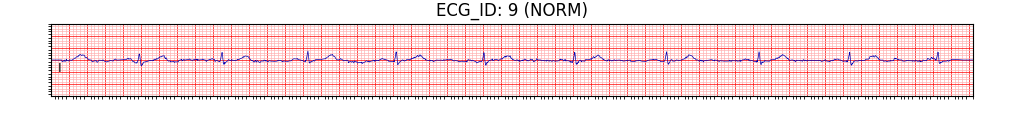
\includegraphics[width=0.95\textwidth]{Imagenes/Vectorial/Transformadas/NORM/ecg.png}
	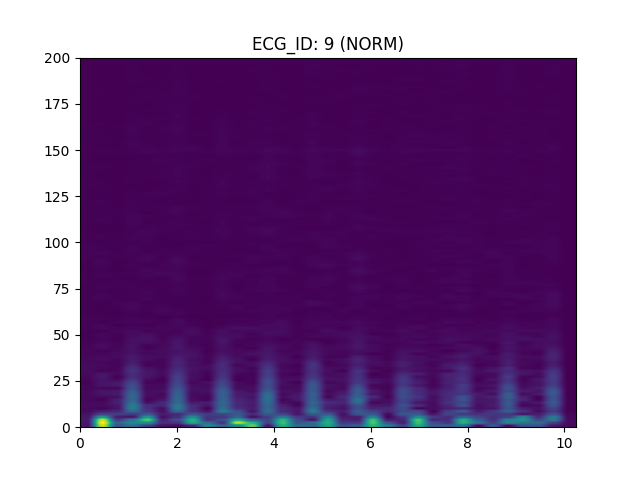
\includegraphics[width=0.45\textwidth]{Imagenes/Vectorial/Transformadas/NORM/stft.png}
	\par Primera derivación de un ECG normal (arriba) y su transformada STFT (abajo).
	\vspace{1cm}
	
	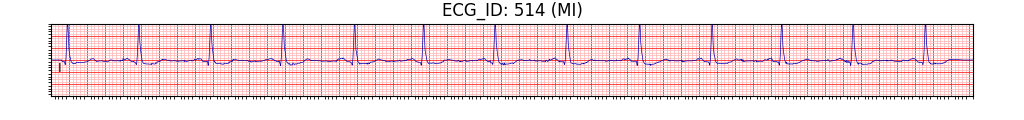
\includegraphics[width=0.95\textwidth]{Imagenes/Vectorial/Transformadas/MI/ecg.png}
	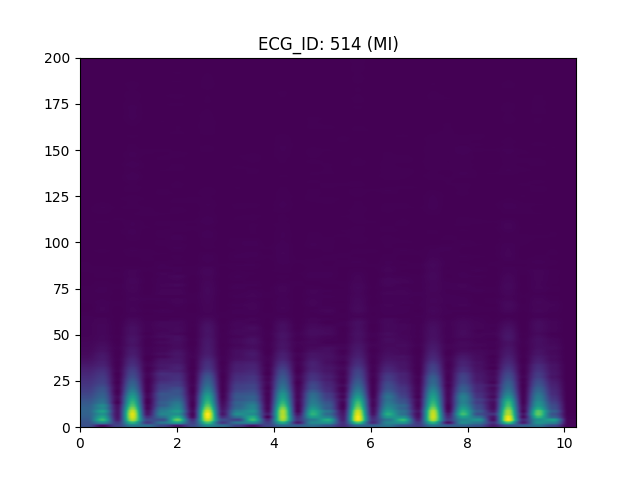
\includegraphics[width=0.45\textwidth]{Imagenes/Vectorial/Transformadas/MI/stft.png}
	\par Primera derivación de un ECG de infarto de miocardio (arriba) y su transformada STFT (abajo).
	\caption{Transformadas STFT de la primera derivación de ECGs para cada clase.}
	\label{fig:stft}
\end{figure}
\begin{figure}[t]\ContinuedFloat
	\centering
	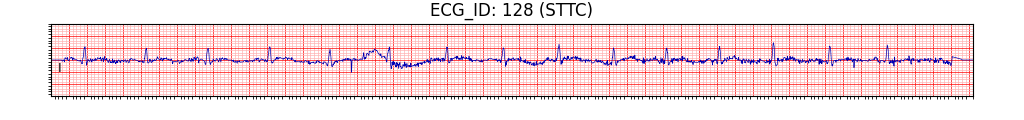
\includegraphics[width=0.95\textwidth]{Imagenes/Vectorial/Transformadas/STTC/ecg.png}
	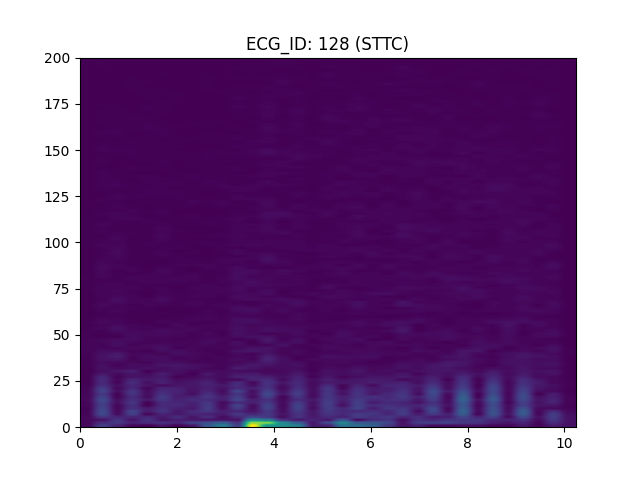
\includegraphics[width=0.45\textwidth]{Imagenes/Vectorial/Transformadas/STTC/stft.png}
	\par Primera derivación de un ECG de tipo STTC (arriba) y su transformada STFT (abajo).
	\vspace{1cm}
		
	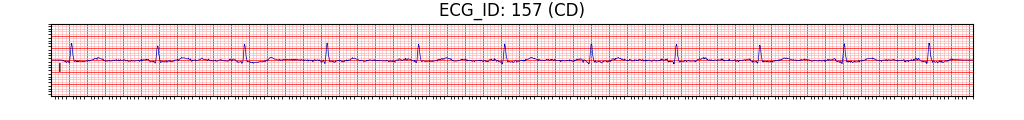
\includegraphics[width=0.95\textwidth]{Imagenes/Vectorial/Transformadas/CD/ecg.png}
	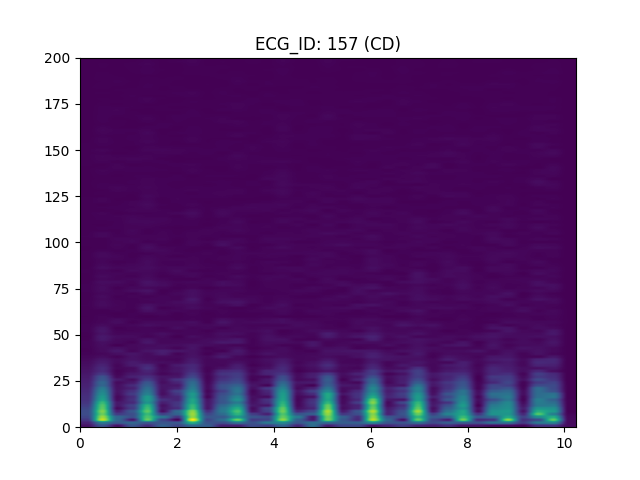
\includegraphics[width=0.45\textwidth]{Imagenes/Vectorial/Transformadas/CD/stft.png}
	\par Primera derivación de un ECG de tipo CD (arriba) y su transformada STFT (abajo).
	\caption{Transformadas STFT de la primera derivación de ECGs para cada clase.}
\end{figure}
\begin{figure}[t]\ContinuedFloat
	\centering
	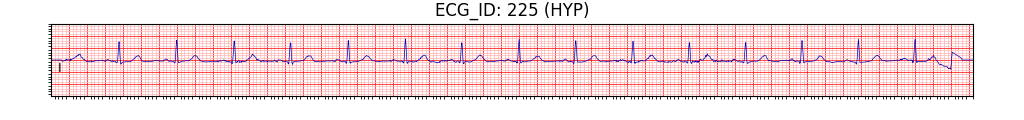
\includegraphics[width=0.95\textwidth]{Imagenes/Vectorial/Transformadas/HYP/ecg.png}
	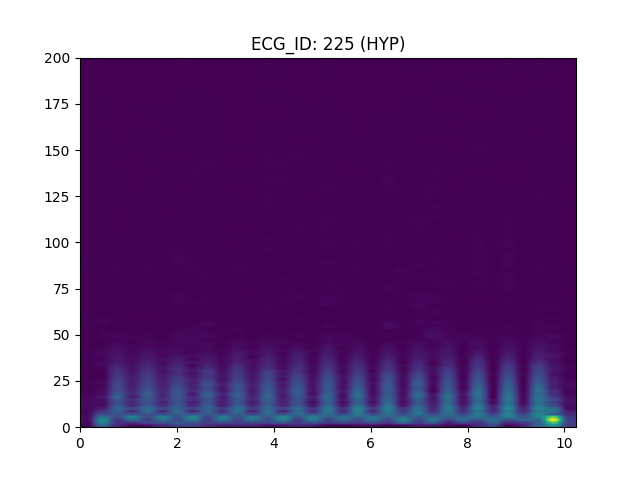
\includegraphics[width=0.45\textwidth]{Imagenes/Vectorial/Transformadas/HYP/stft.png}
	\par Primera derivación de un ECG con hipertrofia (arriba) y su transformada STFT (abajo).
	\caption{Transformadas STFT de la primera derivación de ECGs para cada clase.}
\end{figure}

\subsection{CWT}
\label{subsec:cwt}
La Transformada de Onda Continua (CWT, del inglés \emph{Continous Wavelet Transform}) es una técnica matemática utilizada para analizar señales no estacionarias. A diferencia de la Transformada de Fourier, la CWT descompone la señal en funciones llamadas \emph{wavelets}, que se representan en función de tiempo-frecuencia. Esto (al igual que con la STFT) permite una mayor precisión al estudiar eventos transitorios, ya que las \emph{wavelets} pueden ajustarse para capturar detalles de diferentes escalas temporales o frecuenciales.

La CWT funciona mediante la correlación de la señal original con \emph{wavelets} de diferentes escalas y ubicaciones temporales, lo que permite hacer una representación en el dominio tiempo-frecuencia. A diferencia de la STFT, donde las ventanas tienen un tamaño fijo, la CWT adapta la resolución automáticamente: se utilizan \emph{wavelets} más cortas para capturar detalles de alta frecuencia, mientras que las más largas capturan las características de baja frecuencia. Esto permite un análisis detallado de las señales.

Al aplicar esta transformada, es necesario definir los siguientes parámetros:
\begin{itemize}
	\item \textbf{\emph{Wavelet}}: Es la función base en la que se descompone la señal.
	\item \textbf{Escalas}: Son un conjunto de valores que determinan cómo se dilata (o comprime) la \emph{wavelet} durante el análisis. Están relacionados con la frecuencia de la señal. Las escalas pequeñas corresponden a altas frecuencias mientras que las grandes corresponden a bajas frecuencias.
\end{itemize}

En este trabajo utilizaremos tanto la \emph{wavelet} de Morlet como la de Ricker, ya que ofrecen un buen equilibrio entre localización temporal y frecuencial. Para ambas \emph{wavelets} utilizamos cien valores de escalas, equiespaciadas desde 8 a 637 para la primera y desde 1 a 128 para la segunda.

En la Figura \ref{fig:cwt} se presentan dos ejemplos de transformadas con \emph{wavelet} de Ricker y Morlet respectivamente, con los parámetros que acabamos de elegir. La representación muestra cómo las frecuencias varían a lo largo del tiempo, lo que permite ver eventos específicos como arritmias o cambios en las características de las ondas. Estas visualizaciones pueden ayudar a comprender y analizar los patrones complejos presentes en las señales del ECG con un nivel de detalle que no ofrece la Transformada de Fourier.

\begin{figure}[t]
	\centering
	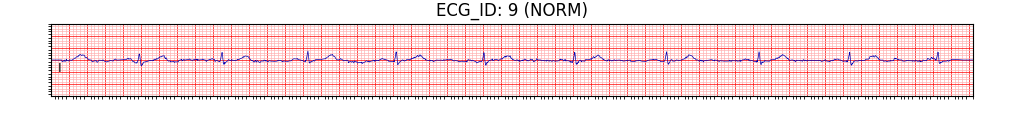
\includegraphics[width=0.95\textwidth]{Imagenes/Vectorial/Transformadas/NORM/ecg.png}
	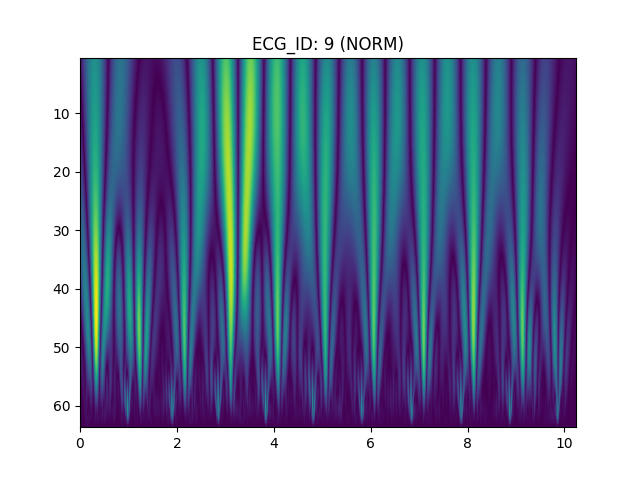
\includegraphics[width=0.45\textwidth]{Imagenes/Vectorial/Transformadas/NORM/cwt_ricker.png}
	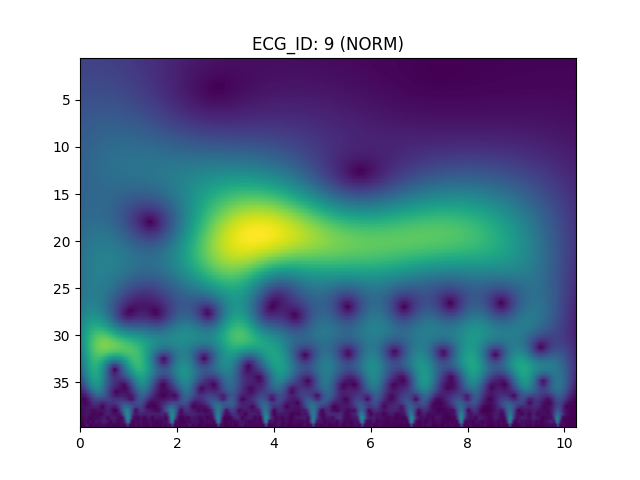
\includegraphics[width=0.45\textwidth]{Imagenes/Vectorial/Transformadas/NORM/cwt_morlet.png}
	\par Primera derivación de un ECG normal (arriba) y su transformada CWT con \emph{wavelet} de Ricker (izquierda) y Morlet (derecha).
	\caption{Transformadas CWT de la primera derivación de ECGs para cada clase.}
	\label{fig:cwt}
\end{figure}
\begin{figure}[t]\ContinuedFloat
	\centering
	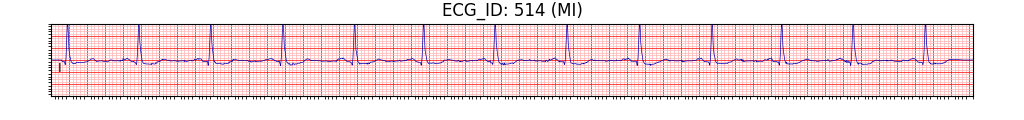
\includegraphics[width=0.95\textwidth]{Imagenes/Vectorial/Transformadas/MI/ecg.png}
	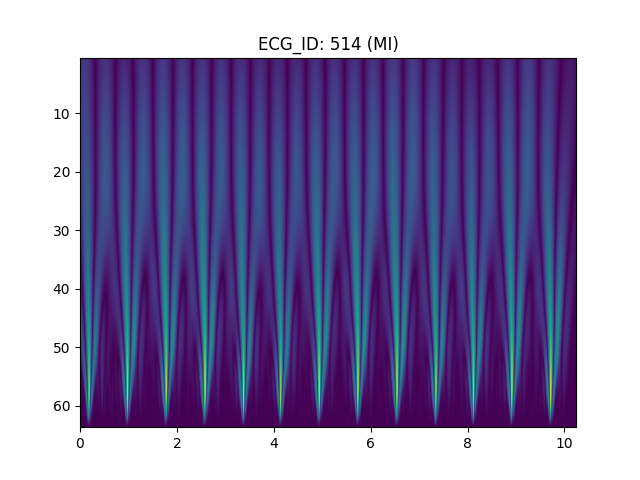
\includegraphics[width=0.45\textwidth]{Imagenes/Vectorial/Transformadas/MI/cwt_ricker.png}
	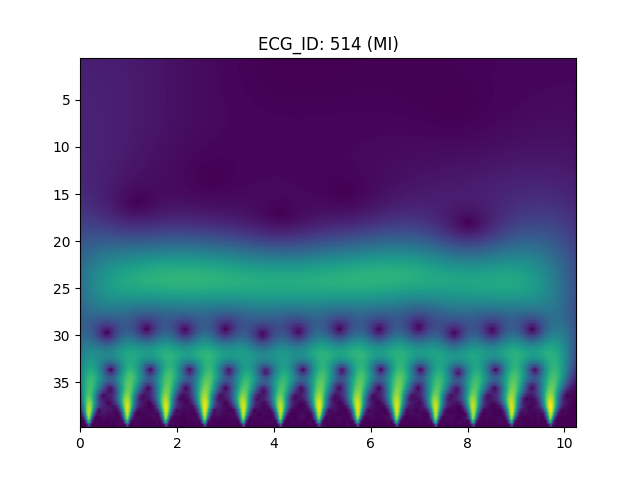
\includegraphics[width=0.45\textwidth]{Imagenes/Vectorial/Transformadas/MI/cwt_morlet.png}
	\par Primera derivación de un ECG de infarto de miocardio (arriba) y su transformada CWT con \emph{wavelet} de Ricker (izquierda) y Morlet (derecha).
	\vspace{1cm}

	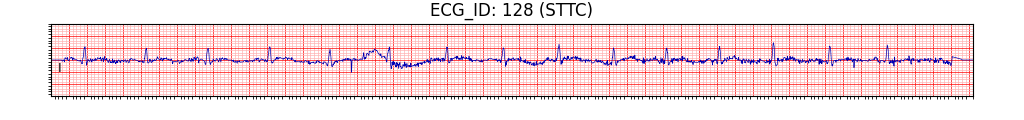
\includegraphics[width=0.95\textwidth]{Imagenes/Vectorial/Transformadas/STTC/ecg.png}
	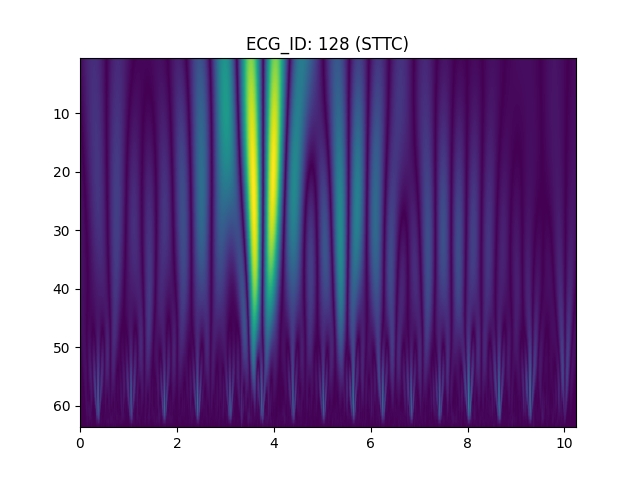
\includegraphics[width=0.45\textwidth]{Imagenes/Vectorial/Transformadas/STTC/cwt_ricker.png}
	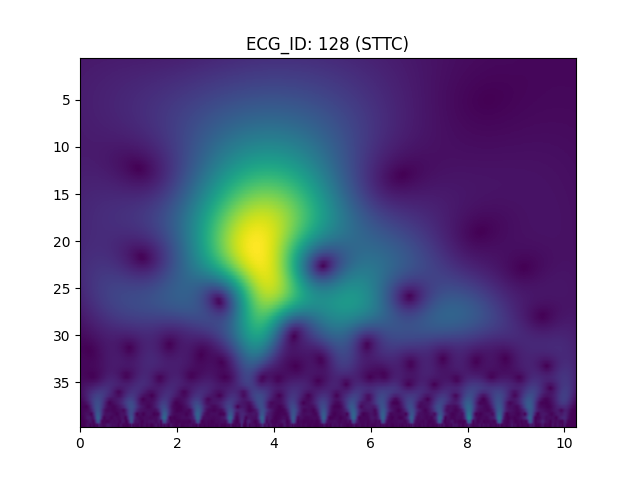
\includegraphics[width=0.45\textwidth]{Imagenes/Vectorial/Transformadas/STTC/cwt_morlet.png}
	\par Primera derivación de un ECG de tipo STTC (arriba) y su transformada CWT con \emph{wavelet} de Ricker (izquierda) y Morlet (derecha).
	\caption{Transformadas CWT de la primera derivación de ECGs para cada clase.}
\end{figure}
\begin{figure}[t]\ContinuedFloat
	\centering
	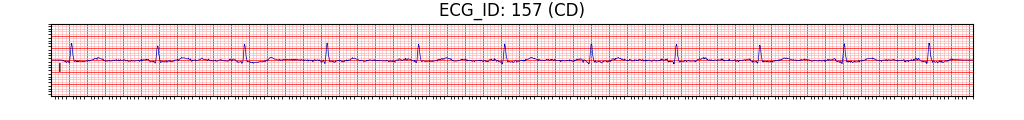
\includegraphics[width=0.95\textwidth]{Imagenes/Vectorial/Transformadas/CD/ecg.png}
	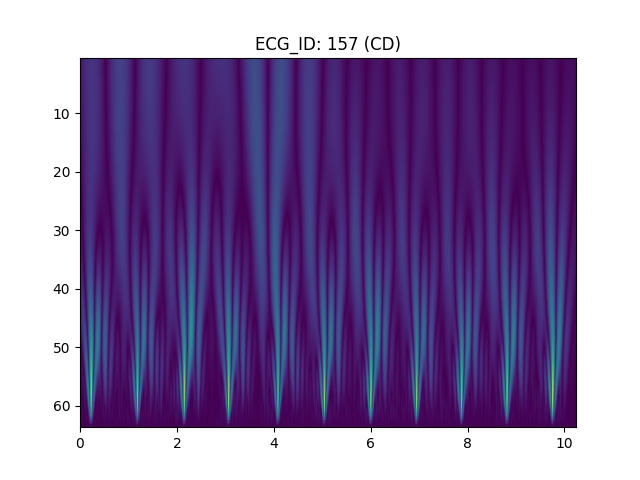
\includegraphics[width=0.45\textwidth]{Imagenes/Vectorial/Transformadas/CD/cwt_ricker.png}
	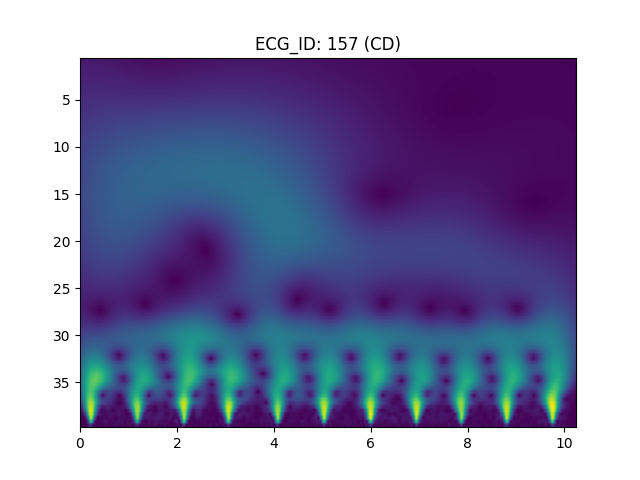
\includegraphics[width=0.45\textwidth]{Imagenes/Vectorial/Transformadas/CD/cwt_morlet.png}
	\par Primera derivación de un ECG de tipo CD (arriba) y su transformada CWT con \emph{wavelet} de Ricker (izquierda) y Morlet (derecha).
	\vspace{1cm}
	
	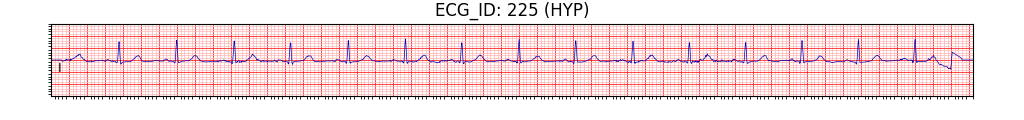
\includegraphics[width=0.95\textwidth]{Imagenes/Vectorial/Transformadas/HYP/ecg.png}
	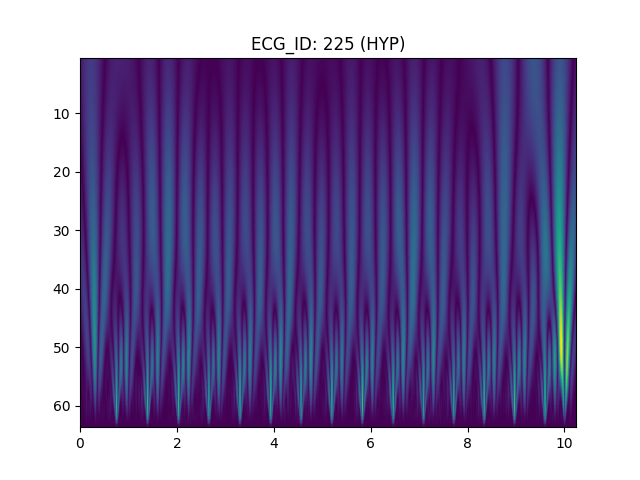
\includegraphics[width=0.45\textwidth]{Imagenes/Vectorial/Transformadas/HYP/cwt_ricker.png}
	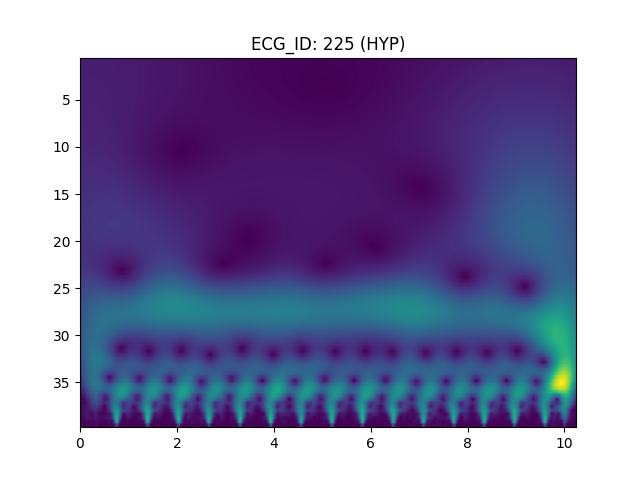
\includegraphics[width=0.45\textwidth]{Imagenes/Vectorial/Transformadas/HYP/cwt_morlet.png}
	\par Primera derivación de un ECG con hipertrofia (arriba) y su transformada CWT con \emph{wavelet} de Ricker (izquierda) y Morlet (derecha).
	\caption{Transformadas CWT de la primera derivación de ECGs para cada clase.}
\end{figure}